%% LyX 2.5.1 created this file.  For more info, see https://www.lyx.org/.
%% Do not edit unless you really know what you are doing.
\documentclass[brazil]{article}
\usepackage[T1]{fontenc}
\usepackage[utf8]{luainputenc}
\usepackage{babel}
\usepackage{amsmath}
\usepackage{amssymb}
\usepackage{graphicx}
\usepackage[]
 {hyperref}

\makeatletter

%%%%%%%%%%%%%%%%%%%%%%%%%%%%%% LyX specific LaTeX commands.

%% Because html converters don't know tabularnewline
\providecommand{\tabularnewline}{\\}

\makeatother

\begin{document}

\section{Abordagem probabilística da lei do valor}
\begin{quote}
Para que os preços a que as mercadorias são trocadas correspondam aproximadamente aos seus valores, nada mais é necessário do que 1) que a troca das várias mercadorias deixe de ser puramente acidental ou apenas ocasional; 2) no que diz respeito à troca direta de mercadorias, que essas mercadorias sejam produzidas em ambos os lados em quantidades aproximadamente suficientes para atender às necessidades mútuas, algo aprendido com a experiência mútua no comércio e, portanto, uma consequência natural do comércio contínuo; e 3) no que diz respeito à venda, que não haja nenhum monopólio natural ou artificial que permita a qualquer uma das partes contratantes vender mercadorias acima de seu valor ou obrigá-las a vender abaixo do valor. Por monopólio acidental entendemos um monopólio que um comprador ou vendedor adquire por meio de uma situação acidental de oferta ou demanda. A suposição de que as mercadorias das várias esferas de produção são vendidas pelo seu valor implica, naturalmente, que o seu valor é o centro de gravidade em torno do qual os seus preços flutuam, e que as suas subidas e descidas contínuas tendem a se equalizar\cite{marx2017capital3}.
\end{quote}

\subsection{Modelagem baseada em agentes}

Este artigo investiga a teoria da lei do valor de Marx utilizando um modelo computacional dinâmico. Ele é apresentado no capítulo 9 do livro ``Econofísica Clássica''\cite{cockshott2012classical} e também no artigo ``A Emergência da Lei do Valor em uma Economia de Mercadoria Simples e Dinâmica''\cite{wright2008emergence}.

Primeiro, devemos estabelecer claramente que existe uma distinção entre valor e preço:
\begin{itemize}
\item \textbf{Valor}: determinado pelas condições técnicas de produção vigentes e mensurado pelo tempo de trabalho socialmente necessário para produzi-lo.
\item \textbf{Preço}: a quantia de dinheiro que a mercadoria rende no mercado.
\end{itemize}
Em uma simplificação teórica do capitalismo (uma ``economia mercantil simples'' ), os preços tendem aos valores, e é isso que queremos demonstrar.

\subsubsection{O modelo}

As características essenciais do modelo são:
\begin{itemize}
\item É composto por $N$ trabalhadores (identificados por um inteiro $i$ entre 1 e N).
\item Existem $L$ mercadorias (identificadas por um inteiro j entre 1 e L).
\item Possui uma quantidade total constante de dinheiro$M=\sum^{N}_{i}m_{i}$.
\item Cada trabalhador produz uma mercadoria por vez.
\item Cada mercadoria é simples: não requer a produção de outra mercadoria e pode ser produzida por um único trabalhador, e todos os trabalhadores produzem a mesma mercadoria com a mesma eficiência.
\item Os agentes produzem para satisfazer suas necessidades.
\end{itemize}

\subsubsection*{Regra de Produção $P_{1}$}
\begin{itemize}
\item No início da simulação, cada agente i possui um vetor $\boldsymbol{e}_{i}=\boldsymbol{0}$ que indica a quantidade de mercadorias que o agente possui.
\item A mercadoria $j$ produzida pelo agente $i$ é dada por $A(i)=j$. Podemos pensar em um vetor $\boldsymbol{A}$ que nos diz o que cada agente está produzindo no momento.
\item Cada mercadoria requer $l_{j}$ passos para ser produzida. Ou seja, a cada passo o agente produz $L_{j}=1/l_{j}$ unidades da mercadoria.
\begin{itemize}
\item Definimos um vetor $\boldsymbol{l}=\left(1/l_{1},\dots,1/l_{L}\right)=\left(L_{1},\dots,L_{L}\right)$.
\end{itemize}
\end{itemize}
Assim, o agente $i$ gera uma unidade da mercadoria $A(i)$ a cada $l_{A(i)}$ passos e, como consequência, o elemento do vetor $e_{i}[A(i)]$ é incrementado em uma unidade.

\subsubsection*{Regra de Consumo $C_{1}$}
\begin{itemize}
\item Todos os agentes têm o mesmo desejo de consumo, dado por um vetor global: $\boldsymbol{c}=\left(1/c_{1},\dots,1/c_{L}\right)=\left(C_{1},\dots,C_{L}\right)$.
\item Cada agente $i$ possui um vetor de déficit de consumo inicializado como $\boldsymbol{d}_{i}=0$.
\item De forma análoga à produção, a cada $c_{j}$ passos, o elemento $\boldsymbol{d}_{i}[j]$ é incrementado em 1, ou seja, a cada passo o desejo do agente aumenta em $C_{j}=1/c_{j}$ unidade.
\end{itemize}
Assim, a cada passo, cad agente consome uma quantidade de mercadorias dada pelo vetor $\boldsymbol{o}_{i}=\text{min}\left(\boldsymbol{e}_{i},\boldsymbol{d}_{i}\right)$. Por exemplo, para a mercadoria $j=1$:
\begin{enumerate}
\item Se o agente não possuir nenhuma mercdoria, $e_{i}[1]=0$, então ele não poderá consumir.
\item Se ele não desejar a mercadoria, $d_{i}[1]=0$, ele também não consumirá.
\item Se ambos os valores forem diferentes de zero e o agente possuir mais do que deseja, $e_{i}[1]>d_{i}[1]$, então ele consumirá apenas o que deseja, $d_{i}[1]$.
\item Mas se o agente tiver menos bens do que deseja, $e_{i}[1]<d_{i}[1]$, ele consumirá tudo o que tiver disponível, $e_{i}[1]$.
\end{enumerate}
Em todos os casos, o consumo é dado pelo menor valor. Evidentemente, essa quantidade consumida deve ser deduzida tanto do déficit quanto dos bens em posse. Assim, os vetores são atualizados como: $\boldsymbol{e}'_{i}=\boldsymbol{e}_{i}-\boldsymbol{o}_{i}$ e $\boldsymbol{d}'_{i}=\boldsymbol{d}_{i}-\boldsymbol{o}_{i}$.

\subsubsection*{Coeficiente de reprodução $\eta=\sum\frac{l_{j}}{c_{j}}$}
\begin{itemize}
\item $\eta=1$ significa que a produção é igual ao consumo: a simulação adotará essa condição.
\item $\eta>1$ significa que a economia está permanentemente em déficit.
\item $\eta<1$ significa que a economia produz permanentemente um excedente.
\end{itemize}
Como em nenhuma circunstância temos $c_{j}<0$ ou $l_{j}<0$, para evitar $\eta>1$ devemos garantir que nenhum termo seja $\frac{l_{j}}{c_{j}}>1$. Se houver mais de uma mercadoria, devemos ser ainda mais restritivos e exigir $\frac{l_{j}}{c_{j}}\leq1$.

Em outras palavras, deve ser necessário menos passos para produzir uma mercadoria do que para desejá-la. Esta é uma condição necessária para a estabilidade, uma vez que cada agente produz apenas uma mercadoria por vez, mas consome todas. Por exemplo, se tivermos duas mercadorias, dois agentes e cada um produzir uma mercadoria com valores $l_{j}=1$ e $c_{j}=2$, então $\eta=0,5+0,5=1$.

\subsubsection*{Regra do preço $O_{1}$}

O preço da mercadoria $j$ de acordo com o agente $i$ é um valor $p^{i}_{j}$ que é sorteado aleatoriamente do intervalo $\left[0,m_{i}\right]$.

\subsubsection*{Regra do Mercado $M_{1}$}

O mercado de uma determinada mercadoria é considerado ``equilibrado'' quando não há mais compradores ou vendedores para essa mercadoria. Em outras palavras, se não estiver equilibrado, significa que ainda existem compradores e vendedores. Começamos com um conjunto $C$ de mercadorias que ainda não foram equilibradas no mercado:
\begin{enumerate}
\item Selecione aleatoriamente uma mercadoria $j$ do conjunto $C$.
\item Selecione aleatoriamente um agente vendedor $s$ do conjunto de vendedores potenciais: isto é, agentes que possuem mais da mercadoria $j$ do que desejam consumir, $e_{i}[j]>d_{i}[j]$.
\item Selecione aleatoriamente um agente comprador $b$ do conjunto de compradores potenciais: isto é, agentes que possuem menos unidades da mercadoria $j$ do que desejam consumir, $e_{i}[j]<d_{i}[j]$.
\item Se não houver compradores ou vendedores potenciais, remova a mercadoria $j$ de $C$. Caso existam, aplique a regra de troca $E_{1}$.
\item Repita os passos anteriores até que todas as mercadorias sejam liquidadas.
\end{enumerate}

\subsubsection*{Regra de troca $E_{1}$}

A regra anterior identifica compradores e vendedores para realizar a troca condicional definida aqui.
\begin{itemize}
\item Uma vez que temos um comprador $b$ e um vendedor $s$ que estimam os preços $p^{b}_{j}$ e $p^{s}_{j}$ para a mercadoria $j$ pela regra $O_{1}$, entõ um preço de transação é extraído do intervalo $\left[p^{b}_{j},p^{s}_{j}\right]$.
\end{itemize}
{*} Se o comprador tiver dinheiro suficiente, a troca ocorre:

o comprador perde dinheiro e ganha uma unidade da mercadoria, enquanto o vendedor ganha dinheiro e perde uma unidade da mercadoria.

\subsubsection*{Regra do Setor $S_{1}$}

Após um período fixo, considerando que estamos no período $n$, cada agente calcula um vetor de erro $\left\Vert \boldsymbol{d}^{n}_{i}\right\Vert $ e o compara com o mesmo vetor calculado no período anterior $\left\Vert \boldsymbol{d}^{n-1}_{i}\right\Vert $. Se o erro aumentou, $\left\Vert \boldsymbol{d}^{n}_{i}\right\Vert >\left\Vert \boldsymbol{d}^{n-1}_{i}\right\Vert $, então o agente muda aleatoriamente a mercadoria que está sendo produzida.

\subsubsection*{Regra de simulação $R_{1}$}

Todo o ciclo de produção, consumo, troca e realocação na produção segue esta regra. Inicialmente, construímos $\boldsymbol{l}$ e $\boldsymbol{c}$ de forma que $\eta=1$, e alocamos $M/N$ entre todos os agentes. Em seguida:
\begin{itemize}
\item Aumentamos o tempo de simulação em um passo.
\item Invocamos a regra $P_{1}$ para cada agente.
\item Invocamos a regra $C_{1}$ para cada agente.
\item Invocamos a regra de mercado $M_{1}$.
\item Invocamos a regra $S_{1}$ para cada agente.
\item Repetimos o processo.
\end{itemize}
Ou seja:

\[
SCE=\left\{ R_{1},P_{1},C_{1},O_{1}\left\{ M_{1},E_{1}\right\} ,S_{1}\right\} 
\]

Os parâmetros são:
\begin{itemize}
\item $N$ --- número de agentes.
\item $L$ --- número de mercadorias.
\item $M$ --- quantia de dinheiro na simulação.
\item $R$ --- o tempo máximo de consumo possível, usado para restringir a construção dos vetores $\boldsymbol{l}$ e $\boldsymbol{c}$.
\item $C$ --- um múltiplo constante de $R$, é um parâmetro que define a duração do período entre aplicações da regra de troca de setor $S_{1}$.
\end{itemize}

\subsubsection{Divisão do trabalho}
\begin{quote}
\textbf{Definição 1}: Uma divisão do trabalho é eficiente quando, para cada mercadoria, a quantidade de mercadorias produzidas é igual à demanda. Assim, a quantidade total da mercadoria $j$ demandada por etapa é $NC_{j}$. Se tivermos uma fração $a_{j}N$ de agentes produzindo a mercadoria $j$, então $a_{j}NL_{j}$ unidades são produzidas por unidade de tempo.
\end{quote}
Para alcançar uma divisão do trabalho eficiente:

\[
a_{j}NL_{j}=NC_{j}\quad\rightarrow\quad a_{j}=\frac{C_{j}}{L_{j}}=\frac{l_{j}}{c_{j}}
\]

Em outras palavras, $a_{j}$ representa uma divisão do trabalho eficiente.

\subsubsection{Preços Objetivos}

Começamos com duas definições:
\begin{itemize}
\item O preço médio da mercadoria $j$ é dado por $\left\langle p_{j}\right\rangle $, e temos o vetor $\boldsymbol{p}=\left(\left\langle p_{1}\right\rangle ,\dots,\left\langle p_{L}\right\rangle \right)$.
\item Os valores, ou seja, a quantidade de tempo investida na produção das mercadorias, são $\boldsymbol{v}=\left(l_{1},\dots,l_{L}\right)$.
\end{itemize}
Assim, se o preço gravita em torno do valor, se é proporcional ao valor, podemos escrever:

\[
\boldsymbol{p}\approx\lambda\boldsymbol{v}
\]

Onde $\lambda$ tem unidades de 'dinheiro por unidade de tempo de trabalho'. Como nossa economia é simples, podemos então definir a Expressão Monetária do Tempo de Trabalho (EMTT) como a razão entre a medida da quantidade total de mercadorias trocadas em um intervalo de tempo a preços correntes e o trabalho produtivo despendido na produção dessas mercadorias.

Em outras palavras, a EMTT é simplesmente:

\[
\lambda=\frac{\gamma M}{\sum l_{i}v_{i}}
\]

Analisando:
\begin{itemize}
\item O numerador é a quantidade de dinheiro trocada em um determinado intervalo de tempo por meio da troca de mercadorias. Aqui, $\gamma$ é simplesmente a proporção de dinheiro trocado por unidade de tempo, então $\gamma M$ é a velocidade da moeda, ou seja, quanto dinheiro é trocado dentro do intervalo de tempo em consideração.
\item O denominador é o trabalho despendido nas mercadorias que são trocadas em um determinado intervalo de tempo. Aqui, $v_{i}$ é a taxa de câmbio média da mercadoria $j$. Assim, temos uma somatória onde cada termo corresponde ao trabalho envolvido nas trocas de cada tipo de mercadoria.
\end{itemize}
Em resumo, temos:

\[
\lambda=\frac{\text{dinheiro trocado por unidade de tempo}}{\text{tempo de trabalho trocado por unidade de tempo}}=\frac{\gamma M}{\sum l_{i}v_{i}}
\]

Evidentemente, estamos focando apenas nas mercadorias que são trocadas, estamos analisando o mercado. Vale ressaltar que, nesse modelo, as mercadorias têm preço apenas no momento da troca, enquanto seu valor é determinado pelas características técnicas de produção de toda a sociedade.

\subsubsection{Simulação}

Nem o livro nem o artigo fornecem o código de implementação exato do modelo, então estou tentando ser o mais fiel possível. A implementação final pode ser conferida no \href{https://github.com/jdansb/Econophysics/blob/main/files/aproximacao_estatistica_da_lei_do_valor_ABM.ipynb}{meu GitHub}. No entanto, após várias semanas trabalhando neste modelo, alguns comentários precisam ser feitos:

\textbf{Comentário 1}: Em nenhum momento é especificado se o dinheiro é inteiro ou não. Apenas é mencionado que o intervalo do qual os preços são extraídos é discreto, o que é um requisito para qualquer modelo computacional, independentemente do tamanho dos intervalos.

A regra de troca pode tornar a execução excessivamente lenta se for usado dinheiro contínuo (usaremos ``contínuo'' para indicar que estamos usando variáveis como float ou double), porque o modelo não avança até que compradores e vendedores cheguem a um acordo para liquidar o mercado. No entanto, se um comprador tiver riqueza próxima de $m_{b}\approx0$, o preço da mercadoria definido pela regra $O_{1}$ precisa estar próximo de 0 para que o agente possa comprar. Quanto maior a riqueza do vendedor, menor a probabilidade disso acontecer.

No apêndice, o livro menciona a implementação de um limite no número de vezes que cada agente pode entrar no mercado, mas não detalha como isso é feito. Optei por usar dinheiro decimal; testes com inteiros produziram resultados mais rápidos, porém menos precisos. Também limitei as visitas dos agentes ao mercado, independentemente do sucesso ou fracasso, ou da mercadoria envolvida. Nos meus testes, aumentar o número de visitas ao mercado até o limite testado tornou o modelo mais preciso, porém mais lento. Contudo, não tenho certeza se permitir tentativas ilimitadas necessariamente melhora os resultados. Seria necessário realizar testes para verificar se a dificuldade de obter a mercadoria desejada por possuir pouca riqueza é um fator importante na dinâmica do sistema.

\textbf{Comentário 2}: Na implementação da regra $S_{1}$ para troca de setores, não está claro como o vetor $\boldsymbol{d}^{(n)}_{i}$ é construído. É simplesmente o vetor $\boldsymbol{d}_{i}$ no último passo do período, ou é um vetor distinto? Optei por esta implementação mais simples mencionada.

Além disso, nesta mesma regra, afirma-se que, se houver um incremento de erro, o agente deve se mover para um ``novo setor'', mas diz-se que o novo setor é sorteado uniformemente entre os $L$ setores. É ambíguo se o agente pode acabar permanecendo no mesmo setor. Implementei de forma que o agente seja forçado a trocar de setor. Alguns testes também sugerem que essa dinâmica de agentes trocando de setor desempenha um papel importante na distribuição de dinheiro entre agentes e setores dentro do sistema, mesmo quando o sistema está em equilíbrio estatístico.

\textbf{Comentário 3}: Não ficou claro para mim o que acontece se, ao aplicar a regra $E_{1}$, a oferta do vendedor $p^{(s)}_{j}$ for maior que a oferta do comprador $p^{(b)}_{j}$. Presumo que sempre consideramos as ofertas do comprador e do vendedor e sorteamos o preço final entre a menor e a maior das duas, independentemente de quem está fazendo a oferta. Na aplicação da regra $O_{1}$, é permitido que uma mercadoria tenha um preço $p=0$. Dependendo do montante total de dinheiro, é altamente possível que uma mercadoria seja trocada sem preço se trabalharmos com números inteiros, o que me parece indesejável.

\textbf{Comentário 4}: Para concluir, devo admitir que tive dificuldades em obter os resultados apresentados para $L>2$. Inicialmente, tentei implementar o código em Python, mas depois migrei para C\# em busca de maior velocidade de execução. Meus resultados mostram uma clara tendência de os preços serem proporcionais ao valor, mas nem sempre com uma correlação tão forte quanto a apresentada no livro e no artigo.

Acredito que, além de algumas possíveis diferenças de implementação, existem certas distribuições de taxas de produção e déficits para as quais o modelo pode apresentar uma taxa de correlação mais alta, e algumas escolhas de parâmetros podem tornar o modelo mais preciso, embora aumentem o custo computacional. Em meus testes, como mencionado, aumentar o número de visitas ao mercado por agente teve um efeito positivo no resultado final. Aumentar o número de agentes em si também ajudou, assim como usar valores monetários contínuos em vez de inteiros. Todas essas decisões melhoram o resultado à custa de um custo computacional maior.

Aumentar a janela de captura de dadosm, por exemplo, calculando a média de 50.000 passos em vez de 5.000, também teve um efeito positivo, novamente ao custo de aumentar o tempo necessário para a simulação ser executada. É por isso que acabei implementando o código em C\#.

No entanto, devo alertar que ainda acredito que possam existir algumas diferenças sutis em comparação com a proposta original, devido à dificuldade de reproduzir fielmente os resultados. A correlação originalmente relatada, mesmo para $L=5$, foi de cerca de 9.8 em 10 execuções, e em um caso chegou a atingir 1. Mesmo assim, acredito que esta versão do modelo já seja suficiente para investigar a questão. Sugestões para melhorias são bem-vindas.

Um dos principais problemas que noto é que a mercadoria com o maior tempo de produção parece ter dificuldade em atingir o preço mais alto. Se tivermos $L=5$, as outras quatro mercadorias seguem uma forte tendência linear, enquanto esta última tem dificuldade em apresentar os resultados esperados. Além disso, esta mercadoria também apresenta um número extremamente baixo de transações, o que acredito ser resultado do déficit acumulado nas etapas anteriores e do fato de o modelo priorizar o consumo em detrimento da troca. Assim, presumo (embora sejam necessárias mais investigações) que os agentes que começam a trabalhar neste setor acabam produzindo mais para consumo do que para troca, ainda mais do que nos outros setores.

Abaixo está um resultado para $L=5$, com $N=200$ agentes, $M=100\cdot N$ e $L\cdot500$ visitas ao mercado por etapa para cada agente, dados obtidos ao longo de 50.000 etapas (50.000-100.000):
\begin{center}
\begin{tabular}{|c|c|c|c|c|}
\hline 
Produto & Preço & Valor & Trocas & Trabalhadores\tabularnewline
\hline 
\hline 
0 & 38,33 & 1.0 & 1975 & 20\tabularnewline
\hline 
1 & 116,84 & 1.5 & 154118 & 30\tabularnewline
\hline 
2 & 553,42 & 2.0 & 22738 & 40\tabularnewline
\hline 
3 & 747,60 & 2.5 & 2207 & 50\tabularnewline
\hline 
4 & 541,66 & 3.0 & 148 & 60\tabularnewline
\hline 
\end{tabular}
\par\end{center}

O preço e a quantidade de trabalhadores são médias e o tempo necessário para aumentar uma unidade de déficit para todas as mercadorias é de $10$. Podemos observar que a distribuição de trabalhadores em cada setor segue a distribuição eficiente e que o preço aumenta com o valor, exceto para a mercadoria de maior valor. No entanto, seu volume de trocas é 13 vezes menor que o da segunda mercadoria de maior valor. Uma mercadoria era trocada aproximadamente a cada 500 passos. Se considerarmos o número de transações por agente, esse número se torna ainda menor. O número de trocas por agente, para cada mercadoria no período é: $[98,75,5137,26,568,45,44,14,2,46]$.

Vale lembrar da passagem no livro que discute os requisitos para a lei do valor operar,
\begin{quote}
{[}se{]} a probabilidade de um vendedor de $j$ encontrar um comprador no mercado for baixa; portanto, a troca se torna ocasional, não atendendo a um requisito para a lei do valor operar\cite{cockshott2012classical}.
\end{quote}
Acredito que seja isso que acontece neste modelo. Apesar de tudo, a relação entre valor e preço permanece clara: se você aumentar o tempo médio de produção de uma mercadoria, o preço médio pelo qual essa mercadoria será negociada tende a aumentar. A correlação considerando todas as mercadorias é de $0,84$ e, desconsiderando a mercadoria de maior valor, é de $0.97$. Devido à natureza estatística do modelo, quando há mais transações, a lei do valor é respeitada.

Para um caso quase idêntico, mas agora permitindo apenas $L\cdot100$ visitas ao mercado por agente, e tomando as médias entre os passos 950.000 e 1.000.000, temos:
\begin{center}
\begin{tabular}{|c|c|c|c|c|}
\hline 
Produto & Preço & Valor & Trocas & Trabalhadores\tabularnewline
\hline 
\hline 
0 & 36,49 & 1.0 & 7151 & 20\tabularnewline
\hline 
1 & 101,88 & 1.5 & 139728 & 30\tabularnewline
\hline 
2 & 547,72 & 2.0 & 17750 & 40\tabularnewline
\hline 
3 & 666,68 & 2.5 & 1226 & 50\tabularnewline
\hline 
4 & 891,73 & 3.0 & 142 & 60\tabularnewline
\hline 
\end{tabular}
\par\end{center}

Uma correlação de $0,97$. Outro indício de que nosso modelo não é totalmente fiel ao livro é que mais da metade das mercadorias têm um preço médio maior que 5 vezes a riqueza per capita. No gráfico apresentado no livro (e no artigo), nenhuma riqueza excede a riqueza per capita. No entanto, acredito que ainda somos capazes de demonstrar a relação entre preço e valor.

Deve-se considerar também que, embora esse resultado seja proporcional, não é necessariamente diretamente proporcional. Ou seja, temos uma espécie de preço base $b$ para a mercadoria, ao qual se adiciona um preço maior de acordo com o tempo de trabalho necessário para produzi-la: $\left\langle p_{j}\right\rangle =\lambda l_{j}+b$.  Para este conjunto de resultados, utilizando um método de regressão linear simples, a relação entre preço e valor pode ser dada pela equação da reta $\left\langle p_{j}\right\rangle =454,98l_{j}-461,01$.
\begin{center}
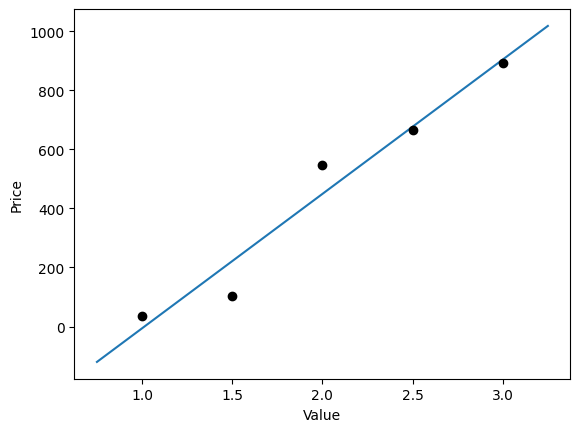
\includegraphics[scale=0.6]{colado8}
\par\end{center}

Poderíamos dedicar tempo a interpretar o que significa esse a existência de um preço base para a mercadoria, mas o ponto mais relevante, para mim, é a inegável relação linear entre preço e valor. Além disso, outras modificações deste modelo podem ser exploradas com o objetivo de corrigir e/ou melhorar os resultados. Exemplos incluem: testar diferentes regras para construir o vetor de déficit a ser aplicado à regra $S_{1}$, ou mesmo uma regra completamente diferente; maneiras alternativas de limitar o número de visitas ao mercado por etapa; limitar o consumo de cada agente por etapa; e assim por diante. Para concluir, podemos analisar um caso especial simples com duas mercadorias, no qual é mais fácil atingir o equilíbrio e podemos alocar trabalhadores de forma eficiente entre os dois setores sem grandes problemas dinâmicos, desativando a regra de troca.
\begin{center}
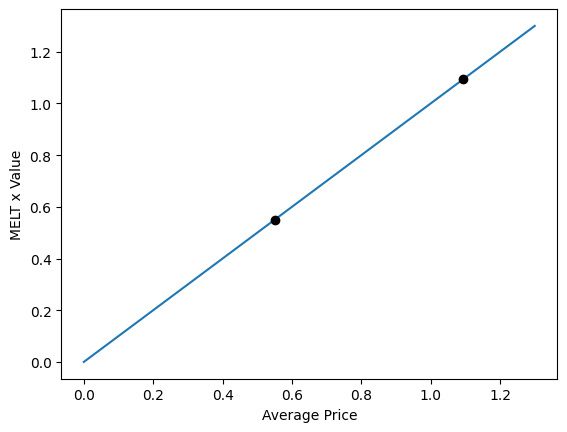
\includegraphics[scale=0.6]{colado9}
\par\end{center}

Essa reta não é o resultado da interpolação dos pontos, mas sim uma reta $y=x$ construída para passar pela origem. Evidentemente, não há vantagem em construir uma reta que passe por dois pontos, mas nada exige que a reta passe pela origem. Isso é uma consequência do modelo.

\subsubsection*{Extra}

Um possível algoritmo para construir os vetores $\boldsymbol{l}$ e $\boldsymbol{c}$ é o seguinte: Primeiro, gere dois vetores aleatórios $\boldsymbol{l}=\left(L_{1},\dots,L_{L}\right)$ e $\boldsymbol{u}=\left(u_{1},\dots,u_{L}\right)$. Então calcule a soma $\sum^{L}_{i}\frac{u_{j}}{L_{j}}=F$. Após isso divida ambos os lados por $F$:

\[
\sum^{L}_{i}\frac{1}{F}\frac{u_{j}}{L_{j}}=\frac{F}{F}\rightarrow\sum^{L}_{i}\frac{u_{j}/F}{L_{j}}=1=\sum^{L}_{i}\frac{C_{j}}{L_{j}}
\]

Ou seja, os elementos do vetor $\boldsymbol{C}$ são $C_{j}=\frac{u_{j}}{F}$, ou equivalentemente, $\boldsymbol{C}=\frac{\boldsymbol{u}}{F}$.

\subsection{Modelagem baseada em equações}

Agora, em vez de um modelo baseado em agentes, temos um modelo baseado em equações. Novamente códigos relacionados à este modelo podem serem encontrados no \href{https://github.com/jdansb/Econophysics/blob/main/files/Statistical_approximation_of_the_law_of_value_(EBM).ipynb}{meu GitHub}.

\subsubsection{Equação do trabalho}

Continuaremos usando as notações matemáticas introduzidas anteriormente e definiremos algumas novas.
\begin{itemize}
\item A velocidade da moeda é dada por $\gamma M$, onde $\gamma$ é uma constante entre 0 e 1.
\item O vetor $\boldsymbol{b}\left(t\right)=\left(b_{1},\dots,b_{L}\right)$ é tal que cada elemento $b_{j}$ representa a fração instantânea (isto é, no instante $t$) do fluxo monetário total recebido pelo setor $j$.
\begin{itemize}
\item Evidentemente, se somarmos todos os setores, teremos $\sum b_{j}=1$.
\end{itemize}
\end{itemize}
Se a velocidade de circulação da moeda $\gamma M$ representa a quantidade total de dinheiro em circulação num dado instante $t$, e $b_{j}$ representa a fração dessa quantidade que o setor $j$ está recebendo, então, claramente, a quantidade total de dinheiro que o setor $j$ está recebendo é dada pelo produto $b_{j}\gamma M$.

O vetor $\boldsymbol{a}\left(t\right)=\left(a_{1},\dots,a_{L}\right)$ é definido de forma que cada elemento $a_{j}$ represente a fração atual de trabalhadores alocados no setor $j$.

Aproximando que, a cada passo, cada agente consome $1/c_{j}$ da mercadoria $j$, e que seu preço médio é $\left\langle p_{j}\right\rangle $, então o custo de consumo atual por passo por agente é $\sum\left\langle p_{j}\right\rangle /c_{j}$.

Consideremos que os agentes trocam de setor com base em um sinal fornecido pelos preços. Isto é, cada setor tem uma taxa de despesa ideal que representa a quantia de dinheiro que precisa ser gasta pelos agentes empregados nesse setor para satisfazer suas necessidades. Essa taxa é dada pelo produto do consumo individual calculado anteriormente e o número atual de agentes trabalhando no setor ($a_{j}N$), ou seja, $a_{j}N\sum\left\langle p_{j}\right\rangle /c_{j}$.

Assim, o fluxo, ou o erro na taxa de rendimento do setor, é dado pela diferença entre o total de dinheiro que entra no setor $j$ e o consumo ideal:

\[
\phi_{j}\left(t\right)=b_{j}\gamma M-a_{j}N\sum^{L}_{k=1}\frac{\left\langle p_{k}\right\rangle }{c_{k}}
\]

Evidentemente, $\phi_{j}>0$ implica que o setor tem lucro, ou seja, o setor recebe mais dinheiro do que os agentes que nele trabalham gastam para satisfazer seu consumo. Por outro lado, $\phi_{j}<0$ implica um déficit, e $\phi_{j}=0$ representa o equilíbrio ideal. Aproximamos então que a troca de agentes entre setores ($da_{j}/dt$) é proporcional a $\phi_{j}$. Por exemplo, se houver um déficit, significa que o setor não tem rendimento suficiente, então os agentes deixarão o setor em busca de outro setor que seja lucrativo e capaz de absorvê-los. Em outras palavras, $da_{j}/dt=\psi\phi_{j}(t)$, onde $\psi$ é uma constante positiva que regula a intensidade da troca de setores.

Esta é a \textbf{equação do trabalho}: ela define como a alocação de trabalho entre diferentes setores de produção varia de acordo com o rendimento recebido pelo setor devido a venda de suas mercadorias. Podemos escrevê-la de forma mais completa:

\[
\frac{da_{j}}{dt}=\psi\phi_{j}\left(t\right)=\psi\left(b_{j}\gamma M-a_{j}N\sum^{L}_{k=1}\frac{\left\langle p_{k}\right\rangle }{c_{k}}\right)
\]

Recordando que o vetor consumo é dado por $\boldsymbol{c}=(1/c_{1},\ldots,1/c_{L})$, e que definimos anteriormente um vetor preço $\boldsymbol{p}=(\left\langle p_{1}\right\rangle ,\ldots,\left\langle p_{L}\right\rangle )$, então $\boldsymbol{c}\cdot\boldsymbol{p}=\sum\frac{\left\langle p_{k}\right\rangle }{c_{k}}$. Assim, a equação do trabalho para toda a economia pode ser escrita em notação vetorial como:

\[
\frac{d\boldsymbol{a}}{dt}=\psi\left(\gamma M\boldsymbol{b}-N\left(\boldsymbol{p}\cdot\boldsymbol{c}\right)\boldsymbol{a}\right)
\]

Agora, como um agente no setor $j$ produz $1/l_{j}$ unidades da mercadoria a cada passo (ela é produzida após $l_{j}$ passos), a produção total no setor em um passo é dada por $a_{j}N/l_{j}$. Se definirmos o preço médio da mercadoria $j$ como o resultado da divisão da renda do setor (como vimos anteriormente, dada por $b_{j}\gamma M$) pela quantidade total de mercadorias produzidas, ou seja, o dinheiro que entrou no setor com a venda de mercadorias dividido pela quantidade de mercadorias produzidas, então o preço médio é:

\[
\left\langle p_{j}\right\rangle =\frac{b_{j}\gamma M}{\frac{a_{j}N}{l_{j}}}=\frac{b_{j}\gamma Ml_{j}}{a_{j}N}=\frac{\gamma M}{N}\frac{b_{j}}{a_{j}}l_{j}
\]


\subsubsection{Equação do dinheiro}

Agora, queremos entender como a variação na renda depende da distribuição do trabalho. Certamente, a renda de um setor depende da quantidade de mercadorias produzidas. Como ninguém consome mais do que precisa, o consumo máximo corresponde à “demanda social” por cada mercadoria $j$.

Como cada agente consome $1/c_{j}$ por passo (ou seja, consome uma unidade da mercadoria a cada $c_{j}$ passos), a demanda social é dada por $N/c_{j}$. Da mesma forma, cada agente empregado no setor $j$ produz $1/l_{j}$, e como o número de agentes no setor é $a_{j}N$, a quantidade total de mercadoria produzida no setor é $a_{j}N/l_{j}$.

Assim, analogamente ao que fizemos anteriormente, o fluxo, ou o erro de produção dado pela diferença entre a quantidade de mercadoria produzida e consumida, é dado por:

\[
\xi_{j}\left(t\right)=\frac{a_{j}N}{l_{j}}-\frac{N}{c_{j}}
\]

Evidentemente, $\xi_{j}>0$ representa superprodução, e $\xi_{j}<0$ implica que a produção é insuficiente, enquanto $\xi_{j}=0$ denota equilíbrio. Se assumirmos que, quando há superprodução (subprodução), o preço cai (sobe), então a variação na renda do setor é proporcional, mas inversamente proporcional, a $\xi_{j}$, ou seja, $db_{j}/dt=-\omega\xi_{j}(t)$, onde $\omega$ é uma constante positiva que ajusta a intensidade com que a distribuição de renda reage ao erro de produção.

Essa equação é conhecida como a \textbf{equação do dinheiro} porque define como a alocação de dinheiro entre diferentes setores varia de acordo com a superprodução ou subprodução de mercadorias. Ela pode ser escrita de forma mais completa como:

\[
\frac{db_{j}}{dt}=-\omega\xi_{j}\left(t\right)=-\omega N\left(\frac{a_{j}}{l_{j}}-\frac{1}{c_{j}}\right)
\]

Se definirmos uma matriz $A$ onde os únicos elementos não nulos são os elementos diagonais $a_{ii}=a_{i}$, e usando o vetor de produção $\boldsymbol{l}=(1/l_{1},...,1/l_{L})$ como um vetor coluna, podemos escrever a equação do dinheiro para toda a economia como:

\[
\frac{d\boldsymbol{b}}{dt}=-N\omega\left(\boldsymbol{A}\boldsymbol{l}-\boldsymbol{c}\right)
\]

Uma vez que o vetor de consumo é $\boldsymbol{c}=(1/c_{1},...,1/c_{L})$. Vamos agora investigar como o equilíbrio deste sistema, formado pelas equações de trabalho e moeda, é alcançado.

\subsubsection{Equilíbrio}

Reunindo os resultados anteriores, temos que um sistema de mercadorias simples é descrito pelo seguinte sistema de equações diferenciais acopladas de ordem $2L$ (a equação do trabalho e a equação monetária para todas as mercadorias):

\begin{align*}
\dot{\boldsymbol{a}} & =\psi\left(\gamma M\boldsymbol{b}-N\left(\boldsymbol{p}\cdot\boldsymbol{c}\right)\boldsymbol{a}\right)\\
\dot{\boldsymbol{b}} & =-\omega N\left(\boldsymbol{A}\boldsymbol{l}-\boldsymbol{c}\right)
\end{align*}

Onde:

\[
\left\langle p_{j}\right\rangle =\frac{\gamma M}{N}\frac{b_{j}}{a_{j}}l_{j}
\]

E com as seguines restrições:

\begin{align*}
\sum^{L}_{j=1}a_{j} & =1 & 0\leq a_{j}\leq1\\
\sum^{L}_{j=1}b_{j} & =1 & 0\leq b_{j}\leq1\\
\sum^{L}_{j=1}\frac{l_{j}}{c_{j}} & =1=\eta & l_{j},c_{j}>0\\
M,N & >0 & \omega,\psi>0\\
0\leq\gamma & \leq1
\end{align*}

Onde: 
\begin{itemize}
\item $M$ ($N$) é a quantidade total de dinheiro (população) no sistema.
\item $a_{j}$ é a fração de trabalhadores produzindo a mercadoria $j$ em um dado momento. 
\begin{itemize}
\item $a_{j}N$ é então o número de trabalhadores no setor $j$, e $\boldsymbol{a}$ é o vetor formado pelos elementos $a_{j}$. Enquanto isso, $\boldsymbol{A}$ é uma matriz onde os únicos elementos não nulos são os elementos diagonais , que são os elementos $a_{i}=a_{ii}$.
\end{itemize}
\item $\gamma$ é a fração de dinheiro trocado por unidade de tempo, então $\gamma M$ é a velocidade do dinheiro.
\item $b_{j}$ é a fração de $\gamma$ recebida pelo setor que produz a mercadoria $j$ em um dado momento, e $\boldsymbol{b}$ é o vetor formado pelos elementos $b_{j}$. 
\item $l_{j}$ ($c_{j}$) é o tempo necessário para que uma mercadoria $j$ seja produzida (consumida).
\begin{itemize}
\item $\boldsymbol{l}$ ($\boldsymbol{c}$) é o vetor formado pelos elementos $1/l_{j}$ ($1/c_{j}$).
\end{itemize}
\item $\omega$ ($\psi$) é uma constante que regula a intensidade com que os trabalhadores (renda) migram entre os setores.
\item $\left\langle p_{j}\right\rangle $ é o preço médio da mercadoria $j$, e $\boldsymbol{p}$ é o vetor formado pelos elementos $\left\langle p_{j}\right\rangle $.
\end{itemize}
Em resumo, este sistema funciona segundo o seguinte esquema: uma determinada divisão do trabalho resulta em superprodução ou subprodução de mercadorias, o que ativa um mecanismo de correção de preços baseado na oferta e na procura. Isso provoca uma alteração na renda do setor, o que, consequentemente, leva os agentes a mudarem de setor, resultando em uma nova divisão do trabalho. Este sistema possui um único ponto de equilíbrio dado por:

\[
\boldsymbol{a}^{*}=\left(\frac{l_{1}}{c_{1}},\dots,\frac{l_{L}}{c_{L}}\right)=\boldsymbol{b}^{*}
\]

Para facilitar a compreensão, vamos revisitar as equações para um único setor $j$:

\begin{align*}
\dot{a}_{j} & =\psi\left(b_{j}\gamma M-a_{j}N\sum^{L}_{k=1}\frac{\left\langle p_{k}\right\rangle }{c_{k}}\right)\\
\dot{b}_{j} & =-\omega N\left(\frac{a_{j}}{l_{j}}-\frac{1}{c_{j}}\right)
\end{align*}

Consideração a situação de equilíbrio, isto é, quando não há mais variações ($\dot{a}_{j}=\dot{b}_{j}=0$):

\begin{align*}
0 & =\psi\left(b^{*}_{j}\gamma M-a^{*}_{j}N\sum^{L}_{k=1}\frac{\left\langle p^{*}_{k}\right\rangle }{c_{k}}\right)\\
0 & =-\omega N\left(\frac{a^{*}_{j}}{l_{j}}-\frac{1}{c_{j}}\right)
\end{align*}

Ou simplesente:

\begin{align*}
0 & =b^{*}_{j}\gamma M-a^{*}_{j}N\sum^{L}_{k=1}\frac{\left\langle p^{*}_{k}\right\rangle }{c_{k}}\\
0 & =\frac{a^{*}_{j}}{l_{j}}-\frac{1}{c_{j}}
\end{align*}

Da segunda equação obtemos direatmente:

\[
a^{*}_{j}=\frac{l_{j}}{c_{j}}
\]

Substituindo na primeira equação, e também usando a definição de preço médio, temos:

\begin{align*}
0 & =b^{*}_{j}\gamma M-\left(a^{*}_{j}\right)N\sum^{L}_{k=1}\frac{1}{c_{k}}\left(\left\langle p^{*}_{k}\right\rangle \right)\\
-b^{*}_{j}\gamma M & =-\left(\frac{l_{j}}{c_{j}}\right)N\sum^{L}_{k=1}\frac{1}{c_{k}}\left(\frac{\gamma M}{N}\frac{b^{*}_{k}}{a^{*}_{k}}l_{k}\right)\\
-b^{*}_{j} & =-\frac{l_{j}}{c_{j}}\sum^{L}_{k=1}\frac{l_{k}}{c_{k}}\frac{b^{*}_{k}}{a^{*}_{k}}
\end{align*}

Substituindo novamente $a^{*}_{j}=\frac{l_{j}}{c_{j}}$ (um termo que reapareceu pois $\left\langle p_{k}\right\rangle $):

\begin{align*}
-b^{*}_{j} & =-\frac{l_{j}}{c_{j}}\sum^{L}_{k=1}\frac{l_{k}}{c_{k}}\frac{1}{a^{*}_{k}}b^{*}_{k}\\
-b^{*}_{j} & =-\frac{l_{j}}{c_{j}}\sum^{L}_{k=1}\frac{l_{k}}{c_{k}}\frac{c_{k}}{l_{k}}b^{*}_{k}\\
-b^{*}_{j} & =-\frac{l_{j}}{c_{j}}\sum^{L}_{k=1}b^{*}_{k}
\end{align*}

E desde que $\sum^{L}_{k=1}b^{*}_{k}=1$, então:

\[
b^{*}_{j}=\frac{l_{j}}{c_{j}}=a^{*}_{j}
\]

Ou seja, quando o sistema está em equilíbrio, a proporção de agentes empregados em cada setor é igual à proporção de dinheiro que cada setor recebe, que é proporcional a $l_{j}/c_{j}$. Isso faz sentido porque todos os agentes neste modelo necessitam da mesma renda para satisfazer suas necessidades. Já mostramos que a divisão eficiente do trabalho ocorre quando $a_{j}=l_{j}/c_{j}$, portanto, um resultado que obtemos sem muito esforço é que, no equilíbrio, a divisão do trabalho tende à eficiência máxima.

Além disso, esse ponto de equilíbrio é assintoticamente estável, isto é, independentemente das condições iniciais, o sistema sempre evolui em direção ao ponto de equilíbrio. Para provar isso, primeiro precisamos a) linearizar o sistema e b) deslocar o ponto de equilíbrio para a origem. Então, podemos aplicar o método direto de Lyapunov. Relembrando que as equações no ponto de equilíbrio são:

\begin{align*}
\dot{a}_{j} & =\psi\gamma Mb_{j}-\psi\sum^{L}_{k=1}\frac{l_{k}\gamma M}{c_{k}}\frac{a_{j}b_{k}}{a_{k}}\\
\dot{b}_{j} & =\frac{\omega N}{c_{j}}-\frac{\omega N}{l_{j}}a_{j}
\end{align*}

Precisamos linearizar o primeiro termo. Primeiro, como $\sum^{L}_{j=1}a_{j}=1$, segue-se que $\sum^{L}_{j=1}\dot{a}_{j}=0$, porque a variação em cada elemento deve ser 'cancelada' por uma variação equivalente de sinal oposto em outro(s) elemento(s) para que a soma permaneça constante. Assim:

\begin{align*}
\dot{a}_{j} & =\psi\gamma Mb_{j}-\psi\sum^{L}_{k=1}\frac{l_{k}\gamma M}{c_{k}}\frac{a_{j}b_{k}}{a_{k}}\\
\sum^{L}_{j=1}\dot{a}_{j} & =\sum^{L}_{j=1}\left[\psi\gamma Mb_{j}-\psi\sum^{L}_{k=1}\frac{l_{k}\gamma M}{c_{k}}\frac{a_{j}b_{k}}{a_{k}}\right]\\
0 & =\sum^{L}_{j=1}b_{j}-\sum^{L}_{j,k=1}\frac{l_{k}}{c_{k}}\frac{a_{j}b_{k}}{a_{k}}\\
\sum^{L}_{j=1}b_{j} & =\sum^{L}_{j,k=1}\frac{l_{j}}{c_{k}}\frac{a_{j}b_{k}}{a_{k}}\\
\left(\sum^{L}_{j=1}b_{j}\right) & =\left(\sum^{L}_{j=1}a_{j}\right)\left(\sum^{L}_{k=1}\frac{l_{k}}{c_{k}}\frac{b_{k}}{a_{k}}\right)\\
1 & =\sum^{L}_{k=1}\frac{l_{k}}{c_{k}}\frac{b_{k}}{a_{k}}
\end{align*}

Onde nós usamos o fato que $\sum^{L}_{j=1}b_{j}=\sum^{L}_{j=1}a_{j}=1$. Revisitando nossa equação então:

\begin{align*}
\dot{a}_{j} & =\psi\gamma Mb_{j}-\psi\sum^{L}_{k=1}\frac{l_{k}\gamma M}{c_{k}}\frac{a_{j}b_{k}}{a_{k}}\\
 & =\psi\gamma Mb_{j}-\psi\gamma Ma_{j}\sum^{L}_{k=1}\frac{l_{k}}{c_{k}}\frac{b_{k}}{a_{k}}\\
 & =\psi\gamma Mb_{j}-\psi\gamma Ma_{j}\psi
\end{align*}

Isto é:

\[
\dot{a}_{j}=\psi\gamma M\left(b_{j}-a_{j}\right)
\]

Agora, com uma simples troca de variáveis $x_{j}=a_{j}-\frac{l_{j}}{c_{j}}$ e $y_{j}=b_{j}-\frac{l_{j}}{c_{j}}$, nós deslocamos o ponto de equilíbrio para a origem. Com essa troca, para a equação do trabalho nós temos:

\begin{align*}
\dot{a}_{j} & =\psi\gamma M\left(b_{j}-a_{j}\right)\\
\frac{d}{dt}\left(x_{j}+\frac{l_{j}}{c_{j}}\right) & =\psi\gamma M\left(\left[y_{j}+\frac{l_{j}}{c_{j}}\right]-\left[x_{j}+\frac{l_{j}}{c_{j}}\right]\right)\\
\dot{x}_{j} & =\psi\gamma M\left(y_{j}-x_{j}\right)
\end{align*}

Ou em notação vetorial:

\[
\dot{\boldsymbol{x}}=\psi\gamma M\left(\boldsymbol{y}-\boldsymbol{x}\right)
\]

E para a equação do dinheiro:

\begin{align*}
\dot{b}_{j} & =-\omega N\left(\frac{a_{j}}{l_{j}}-\frac{1}{c_{j}}\right)\\
\frac{d}{dt}\left(y_{j}+\frac{l_{j}}{c_{j}}\right) & =-\omega N\left(\frac{1}{l_{j}}\left(x_{j}+\frac{l_{j}}{c_{j}}\right)-\frac{1}{c_{j}}\right)\\
\dot{y}_{j} & =-\omega N\left(\frac{x_{j}}{l_{j}}\right)
\end{align*}

Ou em notação veotorial:

\[
\boldsymbol{y}=-\omega n\boldsymbol{X}\boldsymbol{l}
\]

Temos então:

\begin{align*}
\dot{x}_{j} & =\psi\gamma M\left(y_{j}-x_{j}\right)\\
\dot{y}_{j} & =-\omega N\left(\frac{x_{j}}{l_{j}}\right)
\end{align*}

Ou:

\begin{align*}
\dot{\boldsymbol{x}} & =\psi\gamma M\left(\boldsymbol{y}-\boldsymbol{x}\right)\\
\boldsymbol{y} & =-\omega n\boldsymbol{X}\boldsymbol{l}
\end{align*}

Analogamente a $\boldsymbol{A}$, $\boldsymbol{X}$ é a matriz onde apenas os elementos diagonais $x_{ii}$ são diferentes de zero. Como o equilíbrio agora está na origem, os termos $x_{j}$ e $y_{j}$ representam um erro na produção e na renda do setor $j$.

Para formalizar isso, definimos uma função $V:\mathbb{R}^{2L}\rightarrow\mathbb{R}$, que significa que $V$ atribui um número real a cada vetor de variáveis $\left(x_{1},\dots,x_{L},y_{1},\dots,y_{L}\right)$. Essa função nos permite atribuir um valor escalar a cada configuração do sistema. Mais explicitamente:

\[
V\left(x_{1},\dots,x_{L},y_{1},\dots,y_{L}\right)=\frac{1}{2\psi\gamma M}\sum x^{2}_{j}+\frac{1}{2\omega N}\sum l_{j}y^{2}_{j}
\]

Assim, temos uma medida escalar do erro para cada estado possível do nosso sistema. Obviamente, se estivermos na origem, $x_{j}=y_{j}=0$, então $V=0$, e se estivermos longe da origem, então $V>0$, já que $x_{j}$ e $y_{j}$ são números reais maiores ou iguais a zero. Todos os termos são necessariamente não negativos, e a escolha desta forma específica para $V$ visa simplificar os cálculos posteriores.

O que queremos é que $V$ seja uma função de Lyapunov. Para que isso seja possível, $V$ deve primeiro satisfazer $V=0$ na origem e $V>0$ na vizinhança da origem. Como discutido, ambos os casos são satisfeitos com esta definição de $V$. O último requisito é que $\dot{V}\leq0$. Tomando a derivada:

\begin{align*}
\frac{d}{dt}V= & \frac{d}{dt}\left(\frac{1}{2\psi\gamma M}\sum x^{2}_{j}+\frac{1}{2\omega N}\sum l_{j}y^{2}_{j}\right)\\
= & \frac{1}{2\psi\gamma M}\sum\frac{d}{dt}\left(x^{2}_{j}\right)+\frac{1}{2\omega N}\sum l_{j}\frac{d}{dt}\left(y^{2}_{j}\right)\\
= & \frac{1}{2\psi\gamma M}\sum2x_{j}\dot{x}_{j}+\frac{1}{2\omega N}\sum l_{j}2y_{j}\dot{y}_{j}\\
\dot{V}= & \frac{1}{\psi\gamma M}\sum x_{j}\dot{x}_{j}+\frac{1}{\omega N}\sum l_{j}y_{j}\dot{y}_{j}
\end{align*}

Uma vez que a derivada da soma é a soma das derivadas, substituindo $\dot{x}_{j}$ and $\dot{y}_{j}$:

\begin{align*}
\dot{V}= & \frac{1}{\psi\gamma M}\sum x_{j}\dot{x}_{j}+\frac{1}{\omega N}\sum l_{j}y_{j}\dot{y}_{j}\\
= & \frac{1}{\psi\gamma M}\sum x_{j}\left[\psi\gamma M\left(y_{j}-x_{j}\right)\right]+\frac{1}{\omega N}\sum l_{j}y_{j}\left[-\omega N\left(\frac{x_{j}}{l_{j}}\right)\right]\\
= & \sum x_{j}\left(y_{j}-x_{j}\right)-\sum y_{j}x_{j}\\
= & \sum x_{j}y_{j}-\sum x^{2}_{j}-\sum y_{j}x_{j}
\end{align*}

Ou simplesmente:

\[
\dot{V}=-\sum x^{2}_{j}
\]

Evidentemente, $\dot{V}\leq0$, como desejávamos. Além disso, $\dot{V}=0$ ocorre apenas para $\boldsymbol{x}^{*}=0$; em todos os outros casos, temos $\dot{V}<0$. Ou seja, o erro escalar dado por $V$ sempre diminui com o tempo até que o equilíbrio seja alcançado, onde o erro é zero e então se estabiliza. $\dot{V}<0$ na vizinhança do ponto de equilíbrio é o que define um ponto como assintoticamente estável. Nesse caso, como a função de Lyapunov é válida para todo $\mathbb{R}^{2L}$ e não apenas perto do ponto de equilíbrio, podemos dizer que o ponto é globalmente assintoticamente estável.

Finalmente, podemos chegar ao resultado que mais nos interessa: a \textbf{lei do valor}: os valores são atrativos para os preços médios. Ou seja:

\[
\lim_{t\rightarrow\infty}\boldsymbol{p}\left(t\right)=\lambda\boldsymbol{v}
\]

Onde $\boldsymbol{v}=\left(l_{1},\dots,l_{L}\right)$. Como $1/l_{j}$ denota quantas unidades da mercadoria $j$ são produzidas por unidade de tempo, $l_{j}$ denota quantas unidades de tempo são necessárias para produzir a mercadoria $j$. Retornando à definição de preço médio e usando o ponto de equilíbrio ($a_{j}=b_{j}$), temos no equilíbrio:

\[
\left\langle p_{j}\right\rangle =\frac{\gamma M}{N}\frac{b_{j}}{a_{j}}l_{j}=\left(\frac{\gamma M}{N}\right)l_{j}
\]

Temos então $\lambda=\gamma M/N$, representando o valor monetário de uma unidade de tempo de trabalho. À medida que o sistema tende ao equilíbrio, os preços $\boldsymbol{p}$ tendem a $\lambda\boldsymbol{v}$.

É interessante notar que o numerador de $\lambda$ é o mesmo calculado para a simulação: a velocidade da moeda. Mas o denominador é diferente. Devemos lembrar que o denominador representa o trabalho despendido nas mercadorias que são trocadas no mercado durante um determinado intervalo de tempo. Se o nosso intervalo de tempo for de uma unidade, e tivermos $N$ agentes em um sistema onde todos os agentes estão sempre produzindo e trocando o que produziram, então, em uma unidade de tempo, $N$ unidades de tempo de trabalho são incorporadas às mercadorias que foram trocadas.

Isto é, Como estamos analisando apenas os bens que estão sendo trocados no mercado, podemos ver que, em média, $N$ unidades de tempo de trabalho são trocadas por unidade de tempo. Podemos também observar que, de certa forma, quando os agentes mudam de setor buscando maximizar sua renda, eles sempre tentam trabalhar em um setor onde a mercadoria que produzem terá melhor aceitação no mercado. Me parece que aqui a produção é mais orientada a troca.

A solução numérica do sistema para $L$ pode ser vista abaixo demonstrando a evolução do sistema até atingir o equilíbrio estocástico para $\psi=0.1$, $\gamma=0.01$, $M=1.0$, $\omega=0.01$, $N=1.0$, $l=\left(1,2\right)$ e $c=\left(3,3\right)$ ou seja, os pontos de equilíbrio são $l_{1}/c_{1}=0.33$ e o outro $l_{2}/c_{2}=0.67$.
\begin{center}
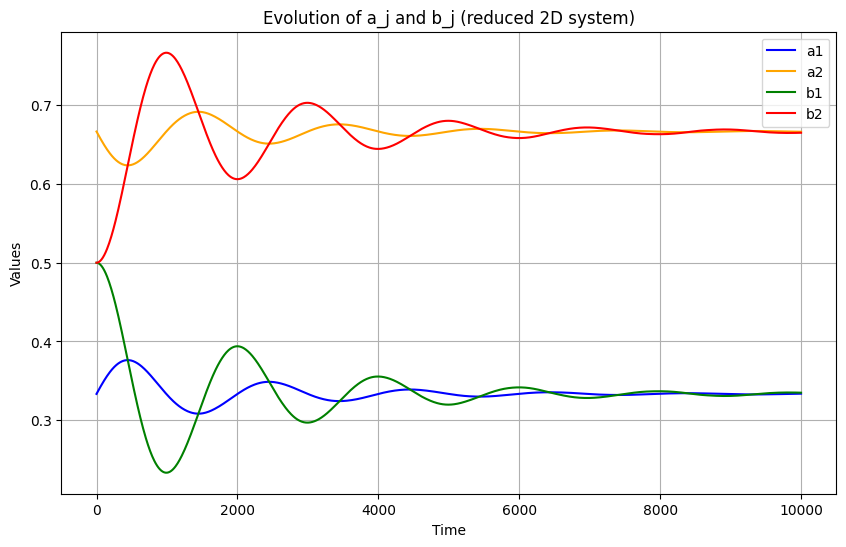
\includegraphics[scale=0.5]{colado10}
\par\end{center}

\subsubsection{Conclusão}

A parte quantitativa da teoria do valor marxista nos diz que os preços estão relacionados ao tempo de trabalho socialmente necessário para produzir uma mercadoria, e os desvios dos preços em relação aos valores são sinais de erros sociais que servem para redistribuir o trabalho. Para analisar isso mais detalhadamente, vamos definir o conceito de trabalho comandado: $\left\langle \epsilon_{j}\right\rangle =\frac{\left\langle p_{j}\right\rangle }{\lambda}$.

Essa quantidade representa quanto tempo de trabalho socialmente necessário, em média, uma mercadoria ``contém'' quando é trocada no mercado. Lembre-se de que a Expressão Monetária do Tempo de Trabalho (EMTT), possui unidades monetárias por unidade de tempo de trabalho. Como o preço é em dinheiro, $\epsilon$ possui unidades de tempo de trabalho. Se $\left\langle \epsilon_{j}\right\rangle <l_{j}$, isso significa que a mercadoria foi negociada a um preço depreciado; de forma oposta, se $\left\langle \epsilon_{j}\right\rangle >l_{j}$, então a mercadoria está sobrevalorizada. Todas essas quantidades são objetivas e independentes de qualquer subjetividade individual sobre a utilidade da mercadoria, e no equilíbrio $\left\langle \epsilon_{j}\right\rangle =l_{j}$.

Manipulando o trabalho necessário, a equação pode ser reescrita como:

\[
\left\langle \epsilon_{j}\right\rangle =\frac{1}{\lambda}\left\langle p_{j}\right\rangle =\frac{N}{\gamma M}\frac{\gamma M}{N}\frac{b_{j}}{a_{j}}l_{j}=\frac{b_{j}}{a_{j}}l_{j}
\]

Isto é, $b_{j}=\left\langle \epsilon_{j}\right\rangle \frac{a_{j}}{l_{j}}$. Substituindo na versão linearizada da equação do trabalho, temos:

\[
\dot{a}_{j}=\psi\gamma M\left(b_{j}-a_{j}\right)=\psi\gamma Ma_{j}\left(\frac{\left\langle \epsilon_{j}\right\rangle }{l_{j}}-1\right)
\]

Ou simplesmente:

\[
\dot{\boldsymbol{a}}=\psi\gamma M\boldsymbol{a}\left(\frac{\left\langle \epsilon_{j}\right\rangle }{l_{j}}-1\right)
\]

Analisando o termo entre parênteses, se $\left(\frac{\left\langle \epsilon_{j}\right\rangle }{l_{j}}>1\right)$, então a subtração é positiva e a mercadoria está sobrevalorizada, sinalizando a necessidade de expandir o setor e aumentar sua produção. Evidentemente, $\left(\frac{\left\langle \epsilon_{j}\right\rangle }{l_{j}}<1\right)$ sinaliza o oposto. Vale ressaltar que o equilíbrio com o qual estamos trabalhando é um equilíbrio estatístico, o que significa que estamos discutindo uma relação média entre valor e preço. Mesmo em equilíbrio, uma transação individual pode ocorrer a preços diferentes. A lei do valor, como apresentada, afirma que, em equilíbrio, o preço médio das mercadorias é proporcional aos seus valores de trabalho.

É importante observar que este modelo não esgota as possibilidades de investigação do tema. Existem modelos que exploram, por exemplo, sistemas de produção complexos onde uma mercadoria é necessária para produzir outra (Krause), mas acredito que, para um primeiro contato, o conteúdo aqui apresentado já cumpre seu propósito.

Se definirmos um coeficiente $\alpha_{ij}$, que indica que 1 hora de trabalho na produção da mercadoria $i$ é equivalente a $\alpha_{ij}$ horas de trabalho na mercadoria $j$, podemos então escrever:

\[
\alpha_{ij}=\frac{\left\langle p_{i}\right\rangle /l_{i}}{\left\langle p_{j}\right\rangle /l_{j}}=\frac{\frac{\gamma M}{N}\frac{b_{i}}{a_{i}}l_{i}/l_{i}}{\frac{\gamma M}{N}\frac{b_{j}}{a_{j}}l_{j}/l_{j}}=\frac{b_{i}/a_{i}}{b_{j}/a_{j}}
\]

Primeiramente, podemos observar que $\frac{\left\langle p_{i}\right\rangle }{l_{i}}$ nos dá a quantia monetária correspondente a uma unidade de tempo de trabalho na produção da mercadoria $i$. Assim, ao dividirmos essa quantia para a mercadoria $i$ pela quantia correspondente para a mercadoria $j$, obtemos o “preço” de uma unidade de tempo de trabalho na produção da mercadoria $i$, expresso como um múltiplo do equivalente para a produção da mercadoria $j$.

Em outras palavras, essa razão “indica que 1 hora de trabalho na produção da mercadoria $i$ é equivalente a $\alpha_{ij}$ horas de trabalho na produção da mercadoria $j$”. Por exemplo, se a mercadoria $i$ tem 2 unidades monetárias por unidade de tempo de trabalho e a mercadoria $j$ tem 4, então $\alpha_{ij}=1/2$, o que significa que para cada intervalo de tempo em que a mercadoria $j$ produz o equivalente a ser vendido como 1 unidade monetária, esse tempo corresponde a $0.5$ unidades monetárias para a mercadoria $i$.

Já obtivemos o resultado de que, no equilíbrio, $a_{j}=b_{j}$, logo, evidentemente, no equilíbrio, $b_{j}/a_{j}=1$, e consequentemente $\alpha_{ij}=1$. Em outras palavras, a afirmação de que os valores são atratores para os preços no equilíbrio é equivalente à afirmação de que os coeficientes homogêneos são atratores para os coeficientes heterogêneos no equilíbrio.

A lei do valor é uma teoria dinâmica da alocação de trabalho baseada na tendência do trabalho heterogêneo de se homogeneizar por meio da troca de mercadorias. Evidentemente, trata-se de um cenário idealizado que nos permite compreender alguns conceitos fundamentais para a análise do capitalismo e está longe de esgotar o assunto.

Em conclusão, a lei do valor é um fenômeno que emerge da interação dinâmica entre produtores privados de mercadorias. No modelo apresentado, os valores são atratores globais para os preços, que por sua vez atuam como sinais de erros que contribuem para uma alocação mais eficiente da divisão social do trabalho disponível entre os setores, e a tendência dos preços a se aproximarem do valor é a expressão monetária da tendência de alocar o trabalho social de forma eficiente. A constante MELT (inglês para EMTT) é interessante porque resume uma relação não óbvia entre um fenômeno de produção (tempo de produção) e um fenômeno de mercado (preços). Com a definição de trabalho comandado, podemos obter um sinal indireto sobre se o trabalho na produção daquela mercadoria é socialmente necessário ou não.

Talvez o mais interessante seja que a lei do valor opera ``nos bastidores''; ela emerge naturalmente da dinâmica do sistema e não precisa ser imposta diretamente em nenhum momento. Vale ressaltar também que o equilíbrio do sistema é estatístico, ou seja, observamos o preço médio de uma mercadoria, que pode ser trocada individualmente a preços diferentes, mesmo quando o sistema atinge o equilíbrio. Além disso, a lei do valor só pode emergir em um sistema econômico que contenha um ciclo de retroalimentação entre produção, consumo, troca e realocação de recursos de trabalho.

\bibliographystyle{plain}
\bibliography{tese,Artigo1/references,Artigo2/referencias}

\end{document}
